%%%%%%%%%%%%%%%%%%%%%%%%%%%%%%%%%%%%%%%%%%%%%%%%%%%%%%%%%%%%%
%% Begin exercise %%
%%%%%%%%%%%%%%%%%%%%%%%%%%%%%%%%%%%%%%%%%%%%%%%%%%%%%%%%%%%%%
\ex{Controlled rectifiers}

%%%%%%%%%%%%%%%%%%%%%%%%%%%%%%%%%%%%%%%%%%%%%%%%%%%%%%%%%%%%%
%% Task 1: M3C converter at a RL-load                     %%
%%%%%%%%%%%%%%%%%%%%%%%%%%%%%%%%%%%%%%%%%%%%%%%%%%%%%%%%%%%%%

\task{M3C converter at an RL-load}
A controlled three-pulse midpoint circuit feeds an ohmic-inductive load. The load inductance $L$ is infinitely large such that a pure direct current $I_\mathrm{2}$ is taken from the converter. The load resistance is $R = \SI{5}{\Omega}$. The converter's ideal transformer is connected to the symmetrical three-phase grid with $U_\mathrm{N} = \SI{230}{\volt} $ (effective value of phase voltage) and  $U_\mathrm{N,LL} = \SI{400}{\volt} $ (line-to-line voltage). The secondary side phase voltages point an effective value of 
$U_{\mathrm{1},i} = \SI{230}{\volt}, \forall i=\mathrm{a,b,c}$. The thyristors and commutation can be assumed to be ideal.

%%%%%%%%%%%%%%%%%%%%%%%%%%%%%%%%%%%%%%%%%%%%%%%%%%%%%%%%%%%%%%%%%%%%%%%
 % M3C rectifier with RL Load
%%%%%%%%%%%%%%%%%%%%%%%%%%%%%%%%%%%%%%%%%%%%%%%%%%%%%%%%%%%%%%%%%%%%%%%
\begin{figure}[htb]
  \begin{center}
    \begin{circuitikz}
      \def\vd{1cm} % vertical distance inductors
      \def\htraf{0.75cm} % horizontal distance transformer coils
      \draw (0,0) to [short, o-] ++(0.5,0) coordinate (L1astart) to [short] ++(0.5,0) to [L] ++(2,0) coordinate (L1aend)
      (0,-1*\vd) to [short, o-] ++(1,0) coordinate (L1bstart) to [L] ++(2,0) coordinate (L1bend)
      (0,-2*\vd) to [short, o-] ++(1,0) coordinate (L1cstart) to [L] ++(2,0) coordinate (L1cend) -- ++(0,-0.5*\vd) to (\tikztostart -| L1astart) 
      to [crossing] ++(0, 1*\vd) to [crossing] ++(0, 1*\vd) to [short, -*] (L1astart)
      (L1aend) -- ++(0,-0.5*\vd) to (\tikztostart -| L1bstart) to [short, -*] (L1bstart)
      (L1bend) -- ++(0,-0.5*\vd) to (\tikztostart -| L1cstart) to [short, -*] (L1cstart);
      \draw let \p1=(L1aend) in (\x1 + \htraf, \y1) coordinate (L2astart) to [L, v^<=$u_{1\mathrm{a}}(t)$, voltage = straight] ++(2,0) to [short, i=$i_{1\mathrm{a}}(t)$] ++(0.5,0) coordinate (L2aend);
      \draw let \p1=(L1bend) in (\x1 + \htraf, \y1) coordinate (L2bstart) to [L, v^<=$u_{1\mathrm{b}}(t)$, voltage = straight] ++(2,0) to [short, i=$i_{1\mathrm{b}}(t)$] ++(0.5,0) coordinate (L2bend);
      \draw let \p1=(L1cend) in (\x1 + \htraf, \y1) coordinate (L2cstart) to [L, v^<=$u_{1\mathrm{c}}(t)$, voltage = straight] ++(2,0) to [short, i=$i_{1\mathrm{c}}(t)$] ++(0.5,0)  coordinate (L2cend);
      \draw (L2astart) to [short, -*] (L2bstart) to [short, -*] (L2cstart) -- ++(0, -1*\vd) -- ++(5,0) coordinate (Rend);
      \draw[double, double distance=3pt, thick] let \p1=(L1aend), \p2=(L2cstart) in (\x1/2+\x2/2, \y1) -- (\x1/2+\x2/2, \y2);
      \draw (L2aend) to [thyristor] ++(1.25,0) coordinate (D1end);
      \draw (L2bend) to [thyristor] ++(1.25,0) coordinate (D2end);
      \draw (L2cend) to [thyristor] ++(1.25,0) coordinate (D3end) to [short, -*] (D2end) to [short, -*] (D1end);
      \draw (D1end) to [short] ++(0.5,0) coordinate (u2) to [short, i=$i_2(t)$] ++(0.75,0) to [L, l=$L$] ++(2,0) coordinate (Ctop) to [short, i = $i_\mathrm{R}(t)$] ++(1.5,0) to [R, l=$R$] (Rend -| \tikztostart) to (Rend); 
      \draw (u2) to [open, v^>=$\hspace{0.5cm}u_2(t)$, voltage = straight] (Rend -| \tikztostart);
    \end{circuitikz}%
  \end{center}
  \caption{M3C topology with an input three-phase transformer and an RL-load.}
  \label{fig:M3C_topology_RL_no_filter}
\end{figure}


% Subtask1
\subtask{Calculate the firing angle $\alpha$ such that an active power of $P = \SI{6}{\kilo\watt}$ is delivered to the load. How big is the resulting load current $i_\mathrm{2}(t) = I_\mathrm{2}$?}
    \begin{solutionblock}
        We can calculate $\bar{u}_\mathrm{2}(\alpha)$ and $I_\mathrm{2}$ from the given active power delivered, $P$, using
        \begin{equation} 
            P = \frac{\bar{u}^2_\mathrm{2}(\alpha)}{R} = \bar{u}_\mathrm{2}(\alpha) I_\mathrm{2},
            \label{sub6.1.1:eq:Active_power_formula}
        \end{equation}
    which would result in 
        \begin{equation}
            \bar{u}_\mathrm{2}(\alpha) \approx \SI{173.2}{\volt},\\
            I_\mathrm{2} \approx \SI{34.6}{\ampere}.
        \end{equation}
        The average output voltage for an arbitrary $\alpha$ is calculated by
        \begin{equation}
            \bar{u}_\mathrm{2}(\alpha) = \frac{3\sqrt{3}}{2\pi}\hat{u}_\mathrm{1}\cos(\alpha),
            \label{sub6.1.1:eq:avg_voltage_alpha}
        \end{equation}
        where
        \begin{equation}
            \hat{u}_\mathrm{1} = \sqrt{2}U_\mathrm{1} = \sqrt{2} 230 \approx \SI{325.27}{\volt}.
            \label{sub6.1.1:eq:voltage_amplitude}
    \end{equation}
    Hence, 
    solving \eqref{sub6.1.1:eq:avg_voltage_alpha} with respect to $\alpha$ results in
        \begin{equation}
            \alpha = \arccos\left(\frac{ 2\pi\bar{u}_\mathrm{2}(\alpha)}{3\sqrt{3}\hat{u}_\mathrm{1}}\right) \approx \SI{0.871}{\radian}.
            \label{sub6.1.1:eq:calculate_alpha}
        \end{equation}    
    
    \end{solutionblock}
% Subtask2
\subtask{Draw the normalized control characteristic curve $\nicefrac{U_\mathrm{2}(\alpha)}{U_\mathrm{2}(\alpha=0)}$ and mark the  operating point $P = \SI{6}{\kilo\watt}$ at $R = \SI{5}{\Omega}$.}
    \begin{solutionblock}
        Substituting $\alpha = 0$ in \eqref{sub6.1.1:eq:avg_voltage_alpha} results in
        \begin{equation}
            \bar{u}_\mathrm{2}(\alpha=0) = \frac{3\sqrt{3}}{2\pi}\hat{u}_\mathrm{1}.
            \label{sub6.1.1:eq:avg_voltage_zero_alpha}
        \end{equation}
        Dividing \eqref{sub6.1.1:eq:avg_voltage_alpha} by \eqref{sub6.1.1:eq:avg_voltage_zero_alpha} leads to  
        \begin{equation}
            \frac{ \bar{u}_\mathrm{2}(\alpha)}{\bar{u}_\mathrm{2}(\alpha=0)} = \cos(\alpha).
            \label{sub6.1.1:eq:voltages_relation}
        \end{equation}    
        %%%%%%%%%%%%%%%%%%%%%%%%%%%%%%%%%%%%%%%%%%%%%%%%%%%%%%%%%%%%%%%%%%%%%%%%%%
% Normalized voltage u_2(alpha)/u_2(alpha=0)
%%%%%%%%%%%%%%%%%%%%%%%%%%%%%%%%%%%%%%%%%%%%%%%%%%%%%%%%%%%%%%%%%%%%%%%%%%
\begin{solutionfigure}[htb]

    %   \documentclass{standalone}
    %   \usepackage{pgfplots}
    %   \pgfplotsset{compat=1.18} % Kompatibilität für neuere Versionen
           \centering
           \begin{tikzpicture}
               \begin{axis}[
                   % x/y range adjustment
                   xmin=0, xmax=180,
                   ymin=-1, ymax=1,
                   samples=500,
                   axis y line=center,
                   axis x line=middle,
                   extra y ticks=0,
                   % Label text
                   xlabel={$\alpha / \text{rad}$},
                   ylabel={$\frac{ U_\mathrm{2}(\alpha)}{U_\mathrm{2}(\alpha=0)}$},
                   % Label adjustment
                   x label style={at={(axis description cs:1,0.4)},anchor=south west},
                   y label style={at={(axis description cs:-.05,.97)},anchor=south,yshift=0.2cm},
                   width=0.6\textwidth,
                   height=0.3\textwidth,
                   % x-Ticks
                   xtick={0,49.9,90,180},
                   xticklabels={0,0.871,$\frac{\pi}{2}$,$\pi$},
                   xticklabel style = {anchor=north},
                   % y-Ticks
                   ytick={-1,-0.5,0,0.5,0.644,1},
                   yticklabels={-1,,0,,0.644,1},
                   yticklabel style = {anchor=east},
                   % Grid layout
                   grid,
                   %grid style={line width=.1pt, draw=gray!10},
                   %major grid style={line width=.2pt,draw=gray!90},
               ]
               % Voltage u_2(alpha)/u_2(alpha=0)
               \addplot[black, domain= 0:180,dashed, thick] {cos(x)}; 
               % u_2(alpha)/u_2(alpha=0) when alpha = 0.87               
               \addplot[color=signalalpha,solid, thick] coordinates{
                (49.9,0)
                (49.9, 0.644)
            };
            \addplot[color=signalalpha,solid, thick] coordinates{
                (0,0.644)
                (49.9, 0.644)
            };
                       
           \end{axis}     
           \end{tikzpicture}
           \caption{Normalized curve for $\frac{ U_\mathrm{2}(\alpha)}{U_\mathrm{2}(\alpha=0)}$ with $\alpha = 0.871$.}
           \label{sfig:ex06_output_voltage_6_1_2}
   \end{solutionfigure}
    \end{solutionblock}
% Subtask3
\subtask{Draw the curve of the converter's output voltage $u_\mathrm{2}(t)$ for the calculated control angle $\alpha$, from subtask 6.1.1, within a plot of the three-phase transformer's secondary voltages.}
    \begin{solutionblock}
        %%%%%%%%%%%%%%%%%%%%%%%%%%%%%%%%%%%%%%%%%%%%%%%%%%%%%%%%%%%%%%%%%%%%%%%%%%
% Output voltage u2 for M3C with RL-Load
%%%%%%%%%%%%%%%%%%%%%%%%%%%%%%%%%%%%%%%%%%%%%%%%%%%%%%%%%%%%%%%%%%%%%%%%%%
\begin{solutionfigure}[htb]

    %   \documentclass{standalone}
    %   \usepackage{pgfplots}
    %   \pgfplotsset{compat=1.18} % Kompatibilität für neuere Versionen
           \centering
           \begin{tikzpicture}
               \begin{axis}[
                   % x/y range adjustment
                   xmin=-90, xmax=368,
                   ymin=-450, ymax=450,
                   samples=500,
                   axis y line=center,
                   axis x line=middle,
                   extra y ticks=0,
                   % Label text
                   xlabel={$\omega t / \text{rad}$},,
                   ylabel={$u/\mathrm{V}$},
                   % Label adjustment
                   x label style={at={(axis description cs:1,0.5)},anchor=west},
                   y label style={at={(axis description cs:-.05,.97)},anchor=south,yshift=0.2cm},
                   width=0.6\textwidth,
                   height=0.3\textwidth,
                   % x-Ticks
                   xtick={-60,0,60,90,180,270,360},
                   xticklabels={$-\frac{\pi}{3}$,,$\frac{\pi}{3}$,,$\pi$,,$2\pi$},
                   xticklabel style = {anchor=north},
                   % y-Ticks
                   ytick={400,200,0,-200,-400},
                   yticklabels={400,200,0,-200,-400},
                   yticklabel style = {anchor=east},
                   % Grid layout
                   grid,
                   %grid style={line width=.1pt, draw=gray!10},
                   %major grid style={line width=.2pt,draw=gray!90},
                   thick
               ]
               % Voltage u1a(wt), u1b(wt) u1c(wt)
               \addplot[black, domain= -90:360,dashed] {325*cos(x)};                
               \addplot[black, domain= -90:360,dashed] {325*cos(x+120)};                
               \addplot[black, domain= -90:360,dashed] {325*cos(x+240)}; 
               % Voltage u2(wt)
               \addplot[signalalpha, domain= -90:-10] {325*cos(x+120)}; 
               \addplot[signalalpha, domain= -10:110] {325*cos(x)};                
               \addplot[signalalpha, domain= 110:230] {325*cos(x+240)};                
               \addplot[signalalpha, domain= 230:350] {325*cos(x+120)};
               \addplot[signalalpha, domain= 350:360] {325*cos(x)}; 
               \addplot[color=signalalpha,solid] coordinates{
                (-10,-111)
                (-10, 317)
            };               
               \addplot[color=signalalpha,solid] coordinates{
                   (110,-111)
                   (110, 317)
               };     
               \addplot[color=signalalpha,solid] coordinates{
                   (230,-111)
                   (230, 317)
               };     
               \addplot[color=signalalpha,solid] coordinates{
                   (350,-111)
                   (350, 317)
               };
        
               % Label of u1c
               \node[black, fill=white, inner sep = 1pt, anchor = south] at (axis cs:340,350) {$u_{\mathrm{1c}}(\omega t)$}; 
               % Label of u1a
               \node[black, fill=white, inner sep = 1pt, anchor = south] at (axis cs:120,350) {$u_{\mathrm{1a}}(\omega t)$};           
               % Label of u1b
               \node[black, fill=white, inner sep = 1pt, anchor = south] at (axis cs:250,350) {$u_{\mathrm{1b}}(\omega t)$};
               % Label of u2
               \node[signalalpha, fill=white, inner sep = 1pt, anchor = south] at (axis cs:180,310) {$u_{\mathrm{2}}(\omega t)$};
               %Label Firing angle 
               \node[black, fill=white, inner sep = 1pt, anchor = south] at (axis cs:80,275){$\alpha$};
               % Line to u2
               \draw[ signalalpha] (185,305) -- (170,230);
               % Line for alpha
               \draw[->](60,270) -- (109.9,270); 
           \end{axis}     
           \end{tikzpicture}
           \caption{Output voltage $u_\mathrm{2}(t)$ for $\alpha = 0.871$.}
           \label{sfig:ex06_output_voltage_6_1_3}
   \end{solutionfigure}
    \end{solutionblock}
% Subtask4
\subtask{Calculate the effective value $I^\mathrm{(1)}_\mathrm{1a}$ of the fundamental current component $i^\mathrm{(1)}_\mathrm{1a}(t)$ and add the latter to the previous plot. How big is the phase shift $\varphi_\mathrm{1a}$ between $u_\mathrm{1a}(t)$ and $i^\mathrm{(1)}_\mathrm{1a}(t)$?}
    \begin{solutionblock}
        Observing the $i_\mathrm{1a}(\omega t)$ signal in Fig. \ref{sfig:ex06_current_signals_6_1_4a}, one can see that it is an even signal. Hence, we expect that the fundamental component of the Fourier Series
        would contain only cosine component ($a_1 \neq 0$) and no sine component ($b_1 = 0$). 
        %%%%%%%%%%%%%%%%%%%%%%%%%%%%%%%%%%%%%%%%%%%%%%%%%%%%%%%%%%%%%%%%%%%%%%%%%%
% Current i_1a(wt)
%%%%%%%%%%%%%%%%%%%%%%%%%%%%%%%%%%%%%%%%%%%%%%%%%%%%%%%%%%%%%%%%%%%%%%%%%%
\begin{solutionfigure}[htb]

    %   \documentclass{standalone}
    %   \usepackage{pgfplots}
    %   \pgfplotsset{compat=1.18} % Kompatibilität für neuere Versionen
           \centering
           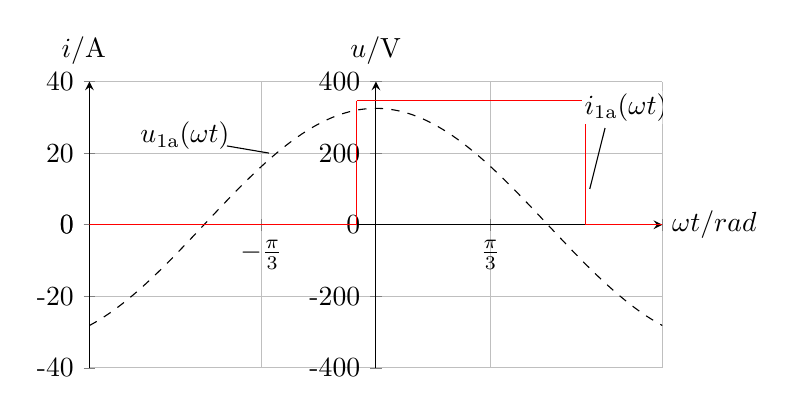
\begin{tikzpicture}
                \pgfplotsset{set layers}
               \begin{axis}[
                   % x/y range adjustment
                   scale only axis,
                   xmin=-150, xmax=150,
                   ymin=-40, ymax=40,
                   samples=500,
                   axis y line=center,
                   axis x line=middle,
                   extra y ticks=0,
                   % Label text
                   xlabel={$\omega t / \text{rad}$},
                   ylabel={$u/\mathrm{V}$},
                   % Label adjustment
                   x label style={at={(axis description cs:1,0.5)},anchor=west},
                   y label style={at={(axis description cs:0.5,.97)},anchor=south,yshift=0.2cm},
                   width=0.6\textwidth,
                   height=0.3\textwidth,
                   % x-Ticks
                   xtick={-150,-60,0,60,150},
                   xticklabels={,$-\frac{\pi}{3}$,0,$\frac{\pi}{3}$,,},
                   xticklabel style = {anchor=north},
                   % y-Ticks
                   ytick={40,20,0,-20,-40},
                   yticklabels={400,200,0,-200,-400},
                   yticklabel style = {anchor=east},
                   % Grid layout
                   grid,
                   %grid style={line width=.1pt, draw=gray!10},
                   %major grid style={line width=.2pt,draw=gray!90},
               ]
               % Voltage u1a(wt)
               \addplot[black, domain= -150:150,dashed] {32.5*cos(x)};
                
                % Label of u1a           
               \node[black, fill=white, inner sep = 1pt, anchor = south] at (axis cs:-100,20) {$u_{\mathrm{1a}}(\omega t)$}; 
               % Line for u1a
               \draw[thin, black] (-78,22) -- (-56,20);
           
           \end{axis}
           \begin{axis}[
            % x/y range adjustment
            scale only axis,
            ymin=-40, ymax=40,
            xmin=-150, xmax=150,
            axis x line=none, 
            samples=500,
            axis y line=left,
            axis x line=middle,
            extra y ticks=0,
            % Label text
            ylabel={$i/\mathrm{A}$},
            % Label adjustment
            y label style={rotate = -90,at={(axis description cs:-0.01,.97)},anchor=south,yshift=0.2cm},
            width=0.6\textwidth,
            height=0.3\textwidth,
            % y-Ticks
            ytick={40,20,0,-20,-40},
            yticklabels={40,20,0,-20,-40},
            yticklabel style = {anchor=east},
            % Grid layout
            grid,
            %grid style={line width=.1pt, draw=gray!10},
            %major grid style={line width=.2pt,draw=gray!90},
        ] 
        % Current i1a(wt)
        \addplot[color=red,solid] coordinates{
            (-150,0)
            (-10.09, 0)
        };                 
           \addplot[color=red,solid] coordinates{
            (-10.09,0)
            (-10.09, 34.6)
        };                   
           \addplot[color=red,solid] coordinates{
               (-10.09,34.6)
               (109.9, 34.6)
           };  
           \addplot[color=red,solid] coordinates{
            (109.9,0)
            (109.9, 34.6)
        };
        \addplot[color=red,solid] coordinates{
            (109.9,0)
            (150, 0)
        };    
           % Label of i1a
           \node[black, fill=white, inner sep = 1pt, anchor = south] at (axis cs:131,28) {$i_{\mathrm{1a}}(\omega t)$};
            % Line to i1a
            \draw[thin, black] (112,10) -- (120,27);
           \end{axis}    
           \end{tikzpicture}
           \caption{Input current $i_\mathrm{1a}(\omega t)$.}
           \label{sfig:ex06_current_signals_6_1_4a}
   \end{solutionfigure}\\
        For simplification, we can position the y-xis in the middle of the conducting period and make use of the period's symmetry. This would simplify the calculations
        by integrating over one half of the period and then multiply by 2. In this case the integration would be from 0 to $\frac{\pi}{3}$, as one conducting
        period is equal to $\frac{2\pi}{3}$. Thus, $a_1$ ($\hat{i}^\mathrm{(1)}_\mathrm{1a}$) can be calculated as:

        \begin{equation}
            a_1 = \hat{i}^\mathrm{(1)}_\mathrm{1a} = \frac{2}{\pi}\int_{0}^{\frac{\pi}{3}}I_\mathrm{2}\cos(\omega t) d\omega t = \left[\frac{2}{\pi} \sin(\omega t)\right]^{\frac{\pi}{3}}_{0} = \frac{1}{\pi}I_\mathrm{2}\sqrt{3}.
            \label{sub6.1.4:eq:calculate_a1}
        \end{equation}  
        
        Then the effective value $I^\mathrm{(1)}_\mathrm{1a}$ is
            \begin{equation}
                I^\mathrm{(1)}_\mathrm{1a} = \frac{\hat{i}^\mathrm{(1)}_\mathrm{1a}}{\sqrt{2}} \approx \SI{13.5}{\ampere}.
                \label{sub6.1.4:eq:calculate_I_rms}
            \end{equation}   
        
        Fig. \ref{sfig:ex06_current_signals_6_1_4b} shows the fundamental component $i^\mathrm{(1)}_\mathrm{1a}(\omega t)$ compared to the input voltage $u_\mathrm{1a}(\omega t)$.
        %%%%%%%%%%%%%%%%%%%%%%%%%%%%%%%%%%%%%%%%%%%%%%%%%%%%%%%%%%%%%%%%%%%%%%%%%%
% Fundamental Current i^1_1a for M3C with RL-Load
%%%%%%%%%%%%%%%%%%%%%%%%%%%%%%%%%%%%%%%%%%%%%%%%%%%%%%%%%%%%%%%%%%%%%%%%%%
\begin{solutionfigure}[htb]

    %   \documentclass{standalone}
    %   \usepackage{pgfplots}
    %   \pgfplotsset{compat=1.18} % Kompatibilität für neuere Versionen
           \centering
           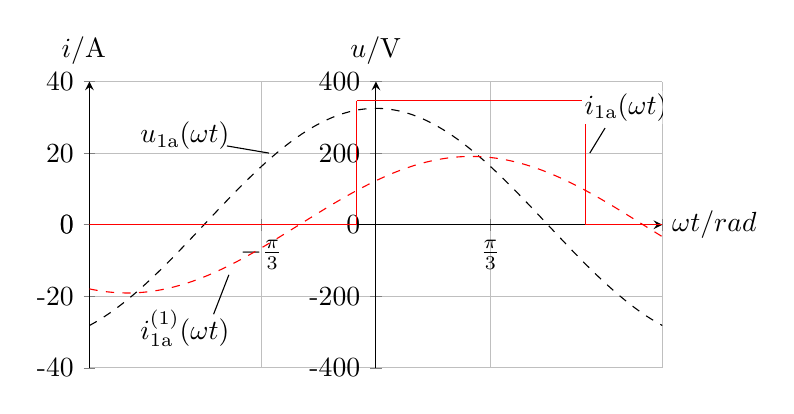
\begin{tikzpicture}
                \pgfplotsset{set layers}
               \begin{axis}[
                    % x/y range adjustment
                    scale only axis,
                    xmin=-150, xmax=150,
                    ymin=-40, ymax=40,
                    samples=500,
                    axis y line=center,
                    axis x line=middle,
                    extra y ticks=0,
                    % Label text
                    xlabel={$\omega t / \text{rad}$},
                    ylabel={$u/\mathrm{V}$},
                    % Label adjustment
                    x label style={at={(axis description cs:1,0.5)},anchor=west},
                    y label style={at={(axis description cs:0.5,.97)},anchor=south,yshift=0.2cm},
                    width=0.6\textwidth,
                    height=0.3\textwidth,
                    % x-Ticks
                    xtick={-150,-60,0,60,150},
                    xticklabels={,$-\frac{\pi}{3}$,0,$\frac{\pi}{3}$,,},
                    xticklabel style = {anchor=north},
                    % y-Ticks
                    ytick={40,20,0,-20,-40},
                    yticklabels={400,200,0,-200,-400},
                    yticklabel style = {anchor=east},
                    % Grid layout
                    grid,
                    %grid style={line width=.1pt, draw=gray!10},
                    %major grid style={line width=.2pt,draw=gray!90},
                ]
               % Voltage u1a(wt)
               \addplot[black, domain= -150:150,dashed] {32.5*cos(x)};
        
            % Label of u1a           
            \node[black, fill=white, inner sep = 1pt, anchor = south] at (axis cs:-100,20) {$u_{\mathrm{1a}}(\omega t)$};
            
            % Line for u1a
            \draw[thin, black] (-78,22) -- (-56,20);
           \end{axis}
           \begin{axis}[
            % x/y range adjustment
            scale only axis,
            ymin=-40, ymax=40,
            xmin=-150, xmax=150,
            axis x line=none, 
            samples=500,
            axis y line=left,
            axis x line=middle,
            extra y ticks=0,
            % Label text
            ylabel={$i/\mathrm{A}$},
            % Label adjustment
            y label style={rotate = -90,at={(axis description cs:-0.01,.97)},anchor=south,yshift=0.2cm},
            width=0.6\textwidth,
            height=0.3\textwidth,
            % y-Ticks
            ytick={40,20,0,-20,-40},
            yticklabels={40,20,0,-20,-40},
            yticklabel style = {anchor=east},
            % Grid layout
            grid,
            %grid style={line width=.1pt, draw=gray!10},
            %major grid style={line width=.2pt,draw=gray!90},
        ] 
        % Current i^1_1a(wt) fundamental
        \addplot[red, domain= -150:150, dashed] {19.07*cos(x-(49.9))};
        % Current i1a(wt)
        \addplot[color=red,solid] coordinates{
            (-150,0)
            (-10.09, 0)
        };                 
           \addplot[color=red,solid] coordinates{
            (-10.09,0)
            (-10.09, 34.6)
        };                   
           \addplot[color=red,solid] coordinates{
               (-10.09,34.6)
               (109.9, 34.6)
           };  
           \addplot[color=red,solid] coordinates{
            (109.9,0)
            (109.9, 34.6)
        };
        \addplot[color=red,solid] coordinates{
            (109.9,0)
            (150, 0)
        };    
           % Label of i1a
           \node[black, fill=white, inner sep = 1pt, anchor = south] at (axis cs:131,28) {$i_{\mathrm{1a}}(\omega t)$};
           % Label of i^1_1a fundamental 
           \node[black, fill=white, inner sep = 1pt, anchor = south] at (axis cs:-100,-35) {$i^\mathrm{(1)}_{\mathrm{1a}}(\omega t)$}; 
            % Line to i1a
            \draw[thin, black] (112,20) -- (120,27);
            % Line to i^1_1a fundamental
            \draw[thin, black] (-85,-25) -- (-77,-14);
           \end{axis}         
           \end{tikzpicture}
           \caption{Fundamental current component $i^\mathrm{(1)}_{\mathrm{1a}}(\omega t)$ for $\alpha = 0.871$.}
           \label{sfig:ex06_current_signals_6_1_4b}
   \end{solutionfigure}\\
        The phase shift of $i^\mathrm{(1)}_\mathrm{1a}(\omega t)$ can be calculated by calculating the phase of the peak of the signal, which can be calculated as: 
        \begin{equation}
            \varphi_\mathrm{1a} = (-\frac{\pi}{3} + \alpha) + (\frac{2\pi}{3} \cdot \frac{1}{2}) = -\frac{\pi}{3} + \alpha + \frac{\pi}{3} = \alpha,   
        \end{equation}
        where -$\frac{\pi}{3} + \alpha$ is the start of the conducting period, while $\frac{2\pi}{3} \cdot \frac{1}{2}$ is half of the period of conduction.
        

    \end{solutionblock}
% Subtask5
\subtask{Calculate the fundamental reactive power $Q^\mathrm{(1)}$ drawn by the converter from the grid.}
    \begin{solutionblock}
        The fundamental reactive power drawn for one full period $(2\pi)$ can be calculated using
        \begin{equation}
            Q^\mathrm{(1)} = 3 U_1 I^\mathrm{(1)}_1 \sin(\alpha)  = 3 \cdot 230 \cdot 13.5 \cdot \sin(0.871) \approx \SI{7.12}{\kilo \volt \ampere}. 
        \end{equation}
    \end{solutionblock}
%%%%%%%%%%%%%%%%%%%%%%%%%%%%%%%%%%%%%%%%%%%%%%%%%%%%%%%%%%%%%
%% Task 2: B6C converter at a motor load                   %%
%%%%%%%%%%%%%%%%%%%%%%%%%%%%%%%%%%%%%%%%%%%%%%%%%%%%%%%%%%%%%
\task{B6C converter at a motor load}

In a lifting drive, a permanent magnet DC motor is supplied by a B6C converter circuit. The B6C-topology is connected to the three-phase grid.
With the assumption of $L\rightarrow\infty$ the motor operates with constant nominal current and constant nominal voltage when lifting as well as lowering the load.
This corresponds to a terminal voltage of $u_\mathrm{mot,up}(t)=U_\mathrm{mot}$ when lifting the load and $u_\mathrm{mot,down}(t)=-U_\mathrm{mot}$ when lowering it.
In order to generate the necessary torque, the motor absorbs the current $i_\mathrm{mot}(t)=I_\mathrm{mot}$.

%%%%%%%%%%%%%%%%%%%%%%%%%%%%%%%%%%%%%%%%%%%%%%%%%%%%%%%%%%%%%%%%%%%%%%%
 % B2U rectifier with capacitive output filtering
%%%%%%%%%%%%%%%%%%%%%%%%%%%%%%%%%%%%%%%%%%%%%%%%%%%%%%%%%%%%%%%%%%%%%%%
    \begin{figure}[htb]
        \begin{center}
            \begin{circuitikz}
                \def\vd{1.5cm} % vertical distance AC sources
                \def\hd{1.5cm} % horizontal distance diode bridge
                \def\h1d{5.0cm} % horizontal position first diode string
                % Base point for voltage supplies
                \coordinate (orig) at (0,0);
                % Voltage sources and neutral connection
                \draw 
                % draw the neutral connection
                (0,0) to [short, -*] ++(0,-1.5) to [short] ++(0,-1.5)
                % draw first phase ua
                (0,0) to [sinusoidal voltage source, v^<=$u_{1\mathrm{a}}$] ++(1.5, 0) to [short, i=$i_{1\mathrm{a}}(t)$]++(0.75,0) -- ++(0.25,0) coordinate (A)
                % draw second phase ub
                (0,-1*\vd) to [sinusoidal voltage source, v^<=$u_{1\mathrm{b}}$] ++(1.5, 0) to [short, i=$i_{1\mathrm{b}}(t)$]++(0.75,0) -- ++(0.25,0) coordinate (B)
                % draw third phase uc
                (0,-2*\vd) to [sinusoidal voltage source, v^<=$u_{1\mathrm{c}}$] ++(1.5,0) to [short, i=$i_{1\mathrm{c}}(t)$]++(0.75,0) -- ++(0.25,0) coordinate (C)
                %thyristor bridge
                % Add thyristor T1
                (\h1d,0) to [thyristor, l=$T_1$, name=D1] ++(0,1.25) coordinate (D1top)
                % Add thyristor T2
                (\h1d,-4.25) coordinate (D2bot) to [thyristor, l=$T_2$, name=D2] ++(0,1.25) to [short] (\h1d, 0)
                % Add connection to junction A
                (\h1d, 0) to [short, *-] (A)
                % Add thyristor T3
                (\h1d+\hd,0) to [thyristor, l=$T_3$, name=D3] ++(0,1.25) coordinate (D3top)
                % Add thyristor T4
                (\h1d+\hd,-4.25) coordinate (D4bot) to [thyristor, l=$T_4$, name=D4] ++(0,1.25) to [short] (\h1d+\hd, 0)
                % Add thyristor T5
                (\h1d+2*\hd,0) to [thyristor, l=$T_5$, name=D5] ++(0,1.25) coordinate (D5top)
                % Add thyristor T6
                (\h1d+2*\hd,-4.25) coordinate (D6bot) to [thyristor, l=$T_6$, name=D6] ++(0,1.25) to [short] (\h1d+2*\hd, 0)
                % Add connection to junction B
                (B -| D3) to [crossing, *-, mirror] ++(-2*\hd,0) -- (B)
                % Add connection to junction C
                (C -| D5) to [short, *-] ++(-\hd/2,0) to [crossing, mirror] ++(-\hd,0) to [crossing, mirror] ++(-\hd,0) -- (C)
                % Add wire T1-T3-T5
                (D1top) to [short, -*] (D3top) to [short, -*] (D5top) to [short, -] ++(0.5,0) coordinate (jL1)
                % Add inductor L and motor current
                (jL1) to [L, l=$L$, name = L] ++(2,0) to [short,i=$\overline{i}_\mathrm{mot}$] ++(0.5,0)  coordinate (jL2)
                % Add DC-motor and motor voltage
                (jL2) to [R, l=$R$, name = R, v_>=$\overline{u}_\mathrm{mot}$, voltage = straight]  (D6bot -| \tikztostart) to (D6bot)
                % Add wire T2-T3-T6
                (D2bot) to [short, -*] (D4bot) to [short, -*] (D6bot)
                % Add voltage arrow u2(t) between Dtop and Dbot
                (jL1) to [open, v^>=$\hspace{0.5cm}u_2(t)$, voltage = straight] (D6bot-|jL1)                
                % Add voltage arrow u2+n(t) between Dtop and neutral
                (D1top) ++(-0.2,0) to [open, v_>=$u_\mathrm{2,p}(t)$, voltage = straight] ++(-5.5,0)
                % Add voltage arrow u2-n(t) between Dbot and neutral
                (D2bot) ++(-0.2,0) to [open, v_>=$u_\mathrm{2,m}(t)$, voltage = straight] ++(-5.5,0)
                % Add voltage arrow between AC source a and b
                (A) to [open, v^>=$\hspace{0.75cm}u_{1\mathrm{ab}}(t)$, voltage = straight] (B)
                % Add voltage arrow between AC source b and c
                (B) to [open, v^>=$\hspace{0.75cm}u_{1\mathrm{bc}}(t)$, voltage = straight] (C)
                % Add voltage arrow between AC source a and c
                (-0.5,-2*\vd) to [open, v^>=$u_{1\mathrm{ca}}(t)\hspace{0.75cm}$, voltage = straight] (-0.5,0);
            \end{circuitikz}
        \end{center}
        \caption{B6C converter at a motor load}
        \label{fig:B6C_topology_WithMotor}
    \end{figure}




\begin{table}[ht]
    \centering  % Zentriert die Tabelle
    \begin{tabular}{ll}
        \toprule
        Input voltages ($i=\mathrm{a,b,c}$): & $U_{\mathrm{1},i}=\SI{230}{\volt}$ (phase voltage) \\
                        & $U_{\mathrm{1,LL},i} = \SI{400}{\volt}$ (line-to-line voltage)\\
        Nom. motor current: & $I_{\mathrm{mot}} = \SI{20}{\ampere}$ \\
        Nom. motor voltage: & $U_\mathrm{mot} = \SI{466}{\volt}$ \\ 
        Grid frequency: & $f= \SI{50}{\hertz}$ \\ 
        \bottomrule
    \end{tabular}
    \caption{Parameters of the lifting drive with B6C converter.}  
    \label{table:ex06_Task2_ParametersOfTheCircuit}
\end{table}


% Subtask1
\subtask{Calculate the firing angle $\alpha_\mathrm{up}$ required for lifting and the firing angle $\alpha_\mathrm{down}$ for lowering the load 
to operate the motor at rated voltage.}
%solution
\begin{solutionblock}
    The average voltage $\overline{u}_\mathrm{2}$ is calculated by
    \begin{equation} 
        \overline{u}_\mathrm{2} = \hat{u}_\mathrm{1,LL} \frac{\pi}{p}\sin(\frac{p}{\pi}) \cos(\alpha).
        \label{eq:ex06t2_u2_gen}
    \end{equation}
    In case of B6C-topology $p$ is equal to 6. The maximum value of $u_\mathrm{1,LL}(t)$ is calculated by
    \begin{equation} 
        \hat{u}_\mathrm{1,LL}=\sqrt{2} \sqrt{3} \cdot U_\mathrm{1}= \sqrt{2} \sqrt{3} \cdot \SI{230}{\volt}=\SI{563}{\volt}.
        \label{eq:ex06t2_u1n_max}
    \end{equation}
    The voltage $\overline{u}_\mathrm{2}$ corresponds to $U_\mathrm{mot}$. Solving \eqref{eq:ex06t2_u2_gen} with respect to $\alpha$ results in
    \begin{equation} 
        \alpha = \arccos( \frac{\overline{u}_\mathrm{2} \cdot p}{\hat{u}_\mathrm{1,LL}\pi \sin(\frac{p}{\pi})})
    \end{equation}
    The following applies to the relevant cases:
    \begin{equation}     
        \begin{split}
            \alpha_\mathrm{up} &= \arccos( \frac{\SI{466}{\volt} \cdot 6}{\SI{563}{\volt}\pi \sin(\frac{6}{\pi})})=\SI{30}{\degree}     \\
            \alpha_\mathrm{down} &= \arccos( \frac{\SI{-466}{\volt} \cdot 6}{\SI{563}{\volt}\pi \sin(\frac{6}{\pi})})=\SI{150}{\degree}    \\
        \end{split}.
        \label{eq:ex06t2_alpha_gen}
    \end{equation}
\end{solutionblock}

% Subtask2
\subtask{Sketch following signals for the two calculated firing angles $\alpha_\mathrm{up}$ and $\alpha_\mathrm{down}$:
\begin{itemize}
    \item The output voltage $u_\mathrm{2,p}(t)$ and $u_\mathrm{2,m}(t)$ of the two partial converters (reference point is neutral)
          and shade the effective voltage-time area for the two cases,
    \item The output voltage $u_\mathrm{2}(t)$ and the mean voltage $\overline{u}_\mathrm{2}$,
    \item The current $i_\mathrm{1a}(t)$ and it's fundamental $i_\mathrm{1a}^{(1)}(t)$,
    \item The voltage of thyristor $u_\mathrm{T1}(t)$,
    \item Indicate which thyristors are conducting during a pulse interval.
\end{itemize}  
}
\begin{solutionblock}
    In \autoref{sfig:ex06_Voltage_u2pm_Up} the output voltages $\overline{u}_\mathrm{2,p}=\SI{233}{\volt}$ and $\overline{u}_\mathrm{2,m}=\SI{-233}{\volt}$
    are entered as dashed blue lines. The ranges in which the respective thyristor conducts are marked with $\mathrm{T_i}$.
    
    %%%%%%%%%%%%%%%%%%%%%%%%%%%%%%%%%%%%%%%%%%%%%%%%%%%%%%%%%%%%%%%%%%%%%%%%%%
% Signals of u2,p u2,m for raising load
%%%%%%%%%%%%%%%%%%%%%%%%%%%%%%%%%%%%%%%%%%%%%%%%%%%%%%%%%%%%%%%%%%%%%%%%%%
\begin{solutionfigure}[htb]

 %   \documentclass{standalone}
 %   \usepackage{pgfplots}
 %   \pgfplotsset{compat=1.18} % Kompatibilität für neuere Versionen
        \centering
        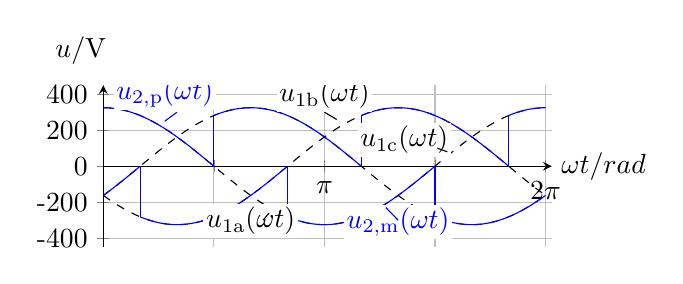
\begin{tikzpicture}
            \begin{axis}[
                % x/y range adjustment
                xmin=0, xmax=365,
                ymin=-450, ymax=450,
                samples=500,
                axis y line=center,
                axis x line=middle,
                extra y ticks=0,
                % Label text
                xlabel={$\omega t / \text{rad}$},,
                ylabel={$u/\mathrm{V}$},
                % Label adjustment
                x label style={at={(axis description cs:1,0.5)},anchor=west},
                y label style={at={(axis description cs:-.05,.97)},anchor=south,yshift=0.2cm},
                width=0.6\textwidth,
                height=0.3\textwidth,
                % x-Ticks
                xtick={0,90,180,270,360},
                xticklabels={,,$\pi$,,$2\pi$},
                xticklabel style = {anchor=north},
                % y-Ticks
                ytick={400,200,0,-200,-400},
                yticklabels={400,200,0,-200,-400},
                yticklabel style = {anchor=east},
                % Grid layout
                grid,
                %grid style={line width=.1pt, draw=gray!10},
                %major grid style={line width=.2pt,draw=gray!90},
            ]
            % Voltage u1a(wt), u1b(wt) u1c(wt)
            \addplot[black, domain= 0:360,dashed] {325*cos(x)};                
            \addplot[black, domain= 0:360,dashed] {325*cos(x+120)};                
            \addplot[black, domain= 0:360,dashed] {325*cos(x+240)}; 
            % Voltage u2p(wt)
            \addplot[blue, domain= 0:90] {325*cos(x)};                
            \addplot[blue, domain= 90:210] {325*cos(x+240)};                
            \addplot[blue, domain= 210:330] {325*cos(x+120)};
            \addplot[blue, domain= 330:360] {325*cos(x)};                
            \addplot[color=blue,solid] coordinates{
                (90,0)
                (90, 281.4)
            };     
            \addplot[color=blue,solid] coordinates{
                (210,0)
                (210, 281.4)
            };     
            \addplot[color=blue,solid] coordinates{
                (330,0)
                (330, 281.4)
            };     
         
            % Voltage u2m(wt)
            \addplot[blue, domain= 0:30] {325*cos(x+240)};                
            \addplot[blue, domain= 30:150] {325*cos(x+120)};                
            \addplot[blue, domain= 150:270] {325*cos(x)};                
            \addplot[blue, domain= 270:360] {325*cos(x+240)};
            \addplot[color=blue,solid] coordinates{
                (30,0)
                (30, -281.4)
            };     
            \addplot[color=blue,solid] coordinates{
                (150,0)
                (150, -281.4)
            };     
            \addplot[color=blue,solid] coordinates{
                (270,0)
                (270, -281.4)
            };     
        
            % Label of u1c
            \node[black, fill=white, inner sep = 1pt, anchor = south] at (axis cs:245,50) {$u_{\mathrm{1c}}(\omega t)$};
            % Line to u1a
            \draw[thin, black] (272,100) -- (280,80); 
            % Label of u1a
            \node[black, fill=white, inner sep = 1pt, anchor = south] at (axis cs:120,-400) {$u_{\mathrm{1a}}(\omega t)$};
            % Line to u1a
            \draw[thin, black] (130,-300) -- (135,-260);            
            % Label of u1b
            \node[black, fill=white, inner sep = 1pt, anchor = south] at (axis cs:180,300) {$u_{\mathrm{1b}}(\omega t)$};
            % Line to u1b
            \draw[thin, black] (180,300) -- (190,260);
            % Label of u2,p
            \node[blue, fill=white, inner sep = 1pt, anchor = south] at (axis cs:50,310) {$u_{\mathrm{2,p}}(\omega t)$};
            % Line to u2,p
            \draw[thin, blue] (60,300) -- (50,250);
            % Label of u2,m
            \node[blue, fill=white, inner sep = 1pt, anchor = south] at (axis cs:240,-410) {$u_{\mathrm{2,m}}(\omega t)$};
            % Line to u2,m
            \draw[thin, blue] (240,-300) -- (230,-230);
        \end{axis}     
        \end{tikzpicture}
        \caption{Output voltage $u_\mathrm{2,p}(t)$ and $u_\mathrm{2,m}(t)$ for raising load.}
        \label{sfig:ex06_Voltage_u2pmn_Raise}
\end{solutionfigure}

    In \autoref{sfig:ex06_Voltage_u2pm_Down} the output voltages are $\overline{u}_\mathrm{2,p}=\SI{-233}{\volt}$ and $\overline{u}_\mathrm{2,m}=\SI{233}{\volt}$.
    
    %%%%%%%%%%%%%%%%%%%%%%%%%%%%%%%%%%%%%%%%%%%%%%%%%%%%%%%%%%%%%%%%%%%%%%%%%%
% Signals of u2,p u2,m for lowing load
%%%%%%%%%%%%%%%%%%%%%%%%%%%%%%%%%%%%%%%%%%%%%%%%%%%%%%%%%%%%%%%%%%%%%%%%%%
\begin{solutionfigure}[htb]

 %   \documentclass{standalone}
 %   \usepackage{pgfplots}
 %   \pgfplotsset{compat=1.18} % Kompatibilität für neuere Versionen
        \centering
        \begin{tikzpicture}
            \begin{axis}[
                % x/y range adjustment
                xmin=0, xmax=368,
                ymin=-500, ymax=500,
                samples=500,
                axis y line=center,
                axis x line=middle,
                extra y ticks=0,
                % Label text
                xlabel={$\omega t / \text{rad}$},,
                ylabel={$u/\mathrm{V}$},
                % Label adjustment
                x label style={at={(axis description cs:1,0.5)},anchor=west},
                y label style={at={(axis description cs:-.05,.97)},anchor=south,yshift=0.2cm},
                width=0.6\textwidth,
                height=0.3\textwidth,
                % x-Ticks
                xtick={0,90,180,270,360},
                xticklabels={,,$\pi$,,$2\pi$},
                xticklabel style = {anchor=north},
                % y-Ticks
                ytick={400,200,0,-200,-400},
                yticklabels={400,200,0,-200,-400},
                yticklabel style = {anchor=east},
                % Grid layout
                grid,
                thick,
                %grid style={line width=.1pt, draw=gray!10},
                %major grid style={line width=.2pt,draw=gray!90},
            ]
            % Voltage u1a(wt), u1b(wt) u1c(wt)
            \addplot[black, domain= 0:360,dashed,name path = u1a] {325*cos(x)};                
            \addplot[black, domain= 0:360,dashed,name path = u1b] {325*cos(x-120)};                
            \addplot[black, domain= 0:360,dashed,name path = u1c] {325*cos(x-240)}; 
            % Voltage u2p(wt)
            \addplot[signalalpha, domain= 0:30] {325*cos(x)};                
            \addplot[signalalpha, domain= 30:150] {325*cos(x-120)};
            \addplot[signalalpha, domain= 150:270] {325*cos(x-240)};                
            \addplot[signalalpha, domain= 270:360] {325*cos(x)};                
            \addplot[color=signalalpha,solid] coordinates{
                (30,0)
                (30, 281.4)
            };     
            \addplot[color=signalalpha,solid] coordinates{
                (150,0)
                (150, 281.4)
            };     
            \addplot[color=signalalpha,solid] coordinates{
                (270,0)
                (270, 281.4)
            };     
    
           % Average u1p 
           \addplot[signalalpha,domain= 0:360,dashed, name path = u2pavg] {-233}; 
            
            % Voltage u2m(wt)
            \addplot[signalalpha, domain= 0:90] {325*cos(x+120)};                
            \addplot[signalalpha, domain= 90:210] {325*cos(x)};                
            \addplot[signalalpha, domain= 210:330] {325*cos(x+240)};
            \addplot[signalalpha, domain= 330:360] {325*cos(x+120)};
            \addplot[color=signalalpha,solid] coordinates{
                (90,0)
                (90, -281.4)
            };     
            \addplot[color=signalalpha,solid] coordinates{
                (210,0)
                (210, -281.4)
            };     
            \addplot[color=signalalpha,solid] coordinates{
                (330,0)
                (330, -281.4)
            };             
 
            % Average u1m 
            \addplot[signalalpha,domain= 0:360,dashed, name path = u2mavg] {233}; 

            % Shade areas of T1,T3,T5
            \addplot[shadecolor, opacity=0.3] fill between[of=u1c and u2pavg, soft clip={domain=0:90}];
            \addplot[shadecolor, opacity=0.3] fill between[of=u1a and u2pavg, soft clip={domain=90:210}];
            \addplot[shadecolor, opacity=0.3] fill between[of=u1b and u2pavg, soft clip={domain=210:330}];
            \addplot[shadecolor, opacity=0.3] fill between[of=u1c and u2pavg, soft clip={domain=330:360}];

            % Shade areas of T2,T4,T5
            \addplot[shadecolor, opacity=0.3] fill between[of=u1a and u2mavg, soft clip={domain=0:30}];
            \addplot[shadecolor, opacity=0.3] fill between[of=u1b and u2mavg, soft clip={domain=30:150}];
            \addplot[shadecolor, opacity=0.3] fill between[of=u1c and u2mavg, soft clip={domain=150:270}];
            \addplot[shadecolor, opacity=0.3] fill between[of=u1a and u2mavg, soft clip={domain=270:360}];            
         
            % Label of u1a
            \node[black, fill=white, inner sep = 1pt, anchor = south] at (axis cs:120,50) {$u_{\mathrm{1a}}(\omega t)$};
            % Line to u1a
            \draw[ black] (90,100) -- (80,80);            
            % Label of u1b
            \node[black, fill=white, inner sep = 1pt, anchor = south] at (axis cs:240,50) {$u_{\mathrm{1b}}(\omega t)$};
            % Line to u1b
            \draw[ black] (210,100) -- (200,80);
            % Label of u1c
            \node[black, fill=white, inner sep = 1pt, anchor = south] at (axis cs:295,-175) {$u_{\mathrm{1c}}(\omega t)$};
            % Line to u1c
            \draw[ black] (265,-120) -- (258,-115);              
            % Label of u2,m
            \node[signalalpha, fill=white, inner sep = 1pt, anchor = south] at (axis cs:50,310) {$u_{\mathrm{2,m}}(\omega t)$};
            % Line to u2,m
            \draw[signalalpha] (60,300) -- (70,250);
            % Label of u2,p
            \node[signalalpha, fill=white, inner sep = 1pt, anchor = south] at (axis cs:240,-410) {$u_{\mathrm{2,p}}(\omega t)$};
            % Line to u2,p
            \draw[signalalpha] (240,-300) -- (250,-230);

            % Thyristor phases u2p
            % Label of T1
            \draw[<->,black, solid] (axis cs:90,-440) -- (axis cs:210,-440);
            \node[black, fill=white, inner sep = 1pt, anchor = south] at (axis cs:170,-500) {$\mathrm{T_1}$};
            % Label of T3
            \draw[<->,black, solid] (axis cs:210,-440) -- (axis cs:330,-440);
            \node[black, fill=white, inner sep = 1pt, anchor = south] at (axis cs:300,-500) {$\mathrm{T_3}$};
            % Label of T5
            \draw[<-,black, solid] (axis cs:330,-440) -- (axis cs:360,-440);
            \draw[->,black, solid] (axis cs:0,-440) -- (axis cs:90,-440);
            \node[black, fill=white, inner sep = 1pt, anchor = south] at (axis cs:30,-500) {$\mathrm{T_5}$};


            % Thyristor phases u2m
            % Label of T4
            \draw[<->,black, solid] (axis cs:30,460) -- (axis cs:150,460);
            \node[black, fill=white, inner sep = 1pt, anchor = south] at (axis cs:100,400) {$\mathrm{T_4}$};
            % Label of T6
            \draw[<->,black, solid] (axis cs:150,460) -- (axis cs:270,460);
            \node[black, fill=white, inner sep = 1pt, anchor = south] at (axis cs:200,400) {$\mathrm{T_6}$};
            % Label of T2
            \draw[<-,black, solid] (axis cs:270,460) -- (axis cs:360,460);
            \draw[->,black, solid] (axis cs:0,460) -- (axis cs:30,460);
            \node[black, fill=white, inner sep = 1pt, anchor = south] at (axis cs:330,400) {$\mathrm{T_2}$};

        \end{axis}     
        \end{tikzpicture}
        \caption{Output voltage $u_\mathrm{2,p}(t)$ and $u_\mathrm{2,m}(t)$ for lowering the load.}
        \label{sfig:ex06_Voltage_u2pm_Down}
\end{solutionfigure}

    

    \FloatBarrier

    In \autoref{sfig:ex06_Voltage_u2up_down} the output voltage $\overline{u}_\mathrm{2}$ is depicted for both cases.

    %%%%%%%%%%%%%%%%%%%%%%%%%%%%%%%%%%%%%%%%%%%%%%%%%%%%%%%%%%%%%%%%%%%%%%%%%%
% Signal of u2 for raising and lowing load
%%%%%%%%%%%%%%%%%%%%%%%%%%%%%%%%%%%%%%%%%%%%%%%%%%%%%%%%%%%%%%%%%%%%%%%%%%
\begin{solutionfigure}[htb]

 %   \documentclass{standalone}
 %   \usepackage{pgfplots}
 %   \pgfplotsset{compat=1.18} % Kompatibilität für neuere Versionen
        \centering
        \begin{tikzpicture}
            \begin{axis}[
                % x/y range adjustment
                xmin=0, xmax=368,
                ymin=-650, ymax=650,
                samples=500,
                axis y line=center,
                axis x line=middle,
                extra y ticks=0,
                % Label text
                xlabel={$\omega t / \text{rad}$},,
                ylabel={$u/\mathrm{V}$},
                % Label adjustment
                x label style={at={(axis description cs:1,0.5)},anchor=west},
                y label style={at={(axis description cs:-.05,.97)},anchor=south,yshift=0.2cm},
                width=0.6\textwidth,
                height=0.3\textwidth,
                % x-Ticks
                xtick={0,90,180,270,360},
                xticklabels={,,$\pi$,,$2\pi$},
                xticklabel style = {anchor=north},
                % y-Ticks
                ytick={600,400,200,0,-200,-400,-600},
                yticklabels={600,400,200,0,-200,-400,-600},
                yticklabel style = {anchor=east},
                % Grid layout
                grid,
                thick
                %grid style={line width=.1pt, draw=gray!10},
                %major grid style={line width=.2pt,draw=gray!90},
            ]
            % Voltage u1ab(wt), u1bc(wt) u1ca(wt)
            \addplot[black, domain= 0:360,dashed] {563*cos(x-30)};                
            \addplot[black, domain= 0:360,dashed] {563*cos(x+90)};                
            \addplot[black, domain= 0:360,dashed] {563*cos(x+210)}; 
            % Voltage -u1ab(wt), -u1bc(wt) -u1ca(wt)
            \addplot[black, domain= 0:360,dashed] {-563*cos(x-30)};                
            \addplot[black, domain= 0:360,dashed] {-563*cos(x+90)};                
            \addplot[black, domain= 0:360,dashed] {-563*cos(x+210)}; 
            % Voltage u2(wt) up
            \addplot[signalalpha, domain= 0:30] {-563*cos(x+210)};            
            \addplot[signalalpha, domain= 30:90] {563*cos(x-30)};                
            \addplot[signalalpha, domain= 270:330] {563*cos(x+90)};                
            \addplot[signalalpha, domain= 150:210] {563*cos(x+210)}; 
            \addplot[signalalpha, domain= 210:270] {-563*cos(x-30)};                
            \addplot[signalalpha, domain= 90:150] {-563*cos(x+90)};                
            \addplot[signalalpha, domain= 330:360] {-563*cos(x+210)};            
            \addplot[color=signalalpha,solid] coordinates{
                (30, 563)
                (30, 282)
            };     
            \addplot[color=signalalpha,solid] coordinates{
                (90, 563)
                (90, 282)
            };     
            \addplot[color=signalalpha,solid] coordinates{
                (150, 563)
                (150, 282)
            };     
            \addplot[color=signalalpha,solid] coordinates{
                (210, 563)
                (210, 282)
            };     
            \addplot[color=signalalpha,solid] coordinates{
                (270, 563)
                (270, 282)
            };     
            \addplot[color=signalalpha,solid] coordinates{
                (330, 563)
                (330, 282)
            };     
    
            % Voltage u2(wt) down
            \addplot[signalalpha, domain= 0:30] {-563*cos(x-30)};                
            \addplot[signalalpha, domain= 150:210] {563*cos(x-30)};                
            \addplot[signalalpha, domain= 30:90] {563*cos(x+90)};                
            \addplot[signalalpha, domain= 270:330] {563*cos(x+210)};            
            \addplot[signalalpha, domain= 330:360] {-563*cos(x-30)};                
            \addplot[signalalpha, domain= 210:270] {-563*cos(x+90)};                
            \addplot[signalalpha, domain= 90:150] {-563*cos(x+210)}; 
            \addplot[color=signalalpha,solid] coordinates{
                (30,-563)
                (30,-282)
            };     
            \addplot[color=signalalpha,solid] coordinates{
                (90,-563)
                (90,-282)
            };     
            \addplot[color=signalalpha,solid] coordinates{
                (150,-563)
                (150,-282)
            };     
            \addplot[color=signalalpha,solid] coordinates{
                (210,-563)
                (210,-282)
            };     
            \addplot[color=signalalpha,solid] coordinates{
                (270,-563)
                (270,-282)
            };     
            \addplot[color=signalalpha,solid] coordinates{
                (330,-563)
                (330,-282)
            };     
         
            % Label of +-u1ab
            \node[black, fill=white, inner sep = 1pt, anchor = south] at (axis cs:30,10) {$\pm u_{\mathrm{1ab}}$};
            % Line to +u1ab
            \draw[black] (30,140) -- (35,190);            
            % Line to -u1ab
            \draw[black] (30,-10) -- (35,-100);            
            % Label of +-u1bc
            \node[black, fill=white, inner sep = 1pt, anchor = south] at (axis cs:150,10) {$\pm u_{\mathrm{1bc}}$};
            % Line to +u1bc
            \draw[black] (150,140) -- (155,190);            
            % Line to -u1bc
            \draw[black] (150,-10) -- (155,-100);   
            % Label of +-u1ca
            \node[black, fill=white, inner sep = 1pt, anchor = south] at (axis cs:270,10) {$\pm u_{\mathrm{1ca}}$};
            % Line to +u1ca
            \draw[black] (270,140) -- (275,190);            
            % Line to -u1ca
            \draw[black] (270,-10) -- (275,-100);               
            % Label of u2up
            \node[signalalpha, fill=white, inner sep = 1pt, anchor = south] at (axis cs:120,210) {$u_{\mathrm{2 up}}$};
            % Line to u2,up
            \draw[signalalpha] (120,370) -- (125,440);
            % Label of u2down
            \node[signalalpha, fill=white, inner sep = 1pt, anchor = south] at (axis cs:240,-380) {$u_{\mathrm{2 dn}}$};
            % Line to u2,down
            \draw[signalalpha] (240,-380) -- (235,-430);
        \end{axis}     
        \end{tikzpicture}
        \caption{Output voltage $u_\mathrm{2 up}(\omega t)$ for raising and $u_\mathrm{2 dn}(\omega t)$ lowering the load.}
        \label{sfig:ex06_Voltage_u2up_down}
\end{solutionfigure}

    \FloatBarrier

    The amplitude of the fundamental $i_\mathrm{1a}^\mathrm{(1)}(t)$ is determined by calculating the Fourier coefficient.
    To simplify the calculation the current signal $i_\mathrm{1a}(t)$ is shift by $\frac{2 \pi}{3}\SI{}{\radian}$ to the left, 
    so that it is axially symmetric. Due to the symmetry the integration is performed only from \SI{0}{\radian} to \SI{\pi}{\radian}:
    \begin{equation}
        \begin{split}
            \hat{i}_\mathrm{1a}^\mathrm{(1)} &= \frac{2}{\pi} \int_{0}^{\pi} i_\mathrm{1a}(\omega t) \cos(\omega t) \mathrm{d}\omega t=
            \frac{2}{\pi} \left( \int_{0}^{\frac{\pi}{3}} I_\mathrm{mot} \cos(\omega t) \mathrm{d}\omega t 
            - \int_{\frac{2\pi}{3}}^{\pi} I_\mathrm{mot} \cos(\omega t) \mathrm{d}\omega t \right)  \\
            &= \frac{2 I_\mathrm{mot}}{\pi} \left( \sin(\frac{\pi}{3}) + \sin(\frac{2\pi}{3}) \right) 
            = \frac{2\cdot \SI{20}{\ampere}}{\pi} \sqrt{3}= \SI{22}{\ampere}.
        \end{split}
    \end{equation}
    The result is valid for raising and lowering the load, because in both cases the current signal 
    forms are identical (except for some phase shift which does not change the fundamental amplitude).

    %%%%%%%%%%%%%%%%%%%%%%%%%%%%%%%%%%%%%%%%%%%%%%%%%%%%%%%%%%%%%%%%%%%%%%%%%%
% Signals of i1a and it's fundamental amplitude for raising load
%%%%%%%%%%%%%%%%%%%%%%%%%%%%%%%%%%%%%%%%%%%%%%%%%%%%%%%%%%%%%%%%%%%%%%%%%%
\begin{solutionfigure}[htb]

 %   \documentclass{standalone}
 %   \usepackage{pgfplots}
 %   \pgfplotsset{compat=1.18} % Kompatibilität für neuere Versionen
        \centering
        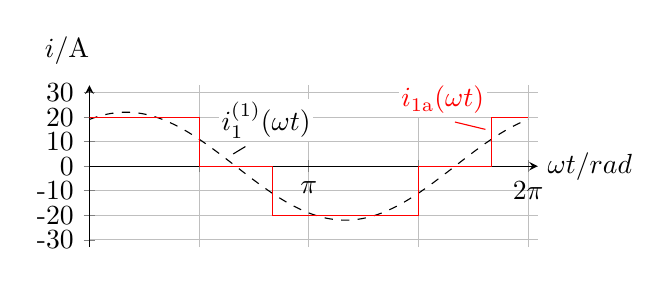
\begin{tikzpicture}
            \begin{axis}[
                % x/y range adjustment
                xmin=0, xmax=368,
                ymin=-33, ymax=33,
                samples=500,
                axis y line=center,
                axis x line=middle,
                extra y ticks=0,
                % Label text
                xlabel={$\omega t / \text{rad}$},,
                ylabel={$i/\mathrm{A}$},
                % Label adjustment
                x label style={at={(axis description cs:1,0.5)},anchor=west},
                y label style={at={(axis description cs:-.05,.97)},anchor=south,yshift=0.2cm},
                width=0.6\textwidth,
                height=0.3\textwidth,
                % x-Ticks
                xtick={0,90,180,270,360},
                xticklabels={,,$\pi$,,$2\pi$},
                xticklabel style = {anchor=north},
                % y-Ticks
                ytick={30,20,10,0,-10,-20,-30},
                yticklabels={30,20,10,0,-10,-20,-30},
                yticklabel style = {anchor=east},
                % Grid layout
                grid,
                %grid style={line width=.1pt, draw=gray!10},
                %major grid style={line width=.2pt,draw=gray!90},
            ]
            % Current i1 fundamentel
            \addplot[black, domain= 0:360,dashed] {22*cos(x-30)};                
            % Current i1d
            \addplot[color=red,solid] coordinates{
                (0, 20)
                (90, 20)
                (90, 0)
                (150, 0)
                (150, -20)
                (270, -20)
                (270, 0)
                (330, 0)
                (330, 20)
                (360, 20)
            };     
        
            % Label of i1a
            \node[red, fill=white, inner sep = 1pt, anchor = south] at (axis cs:290,20) {$i_{\mathrm{1a}}(\omega t)$};
            % Line to i1a
            \draw[thin, red] (325,15) -- (300,18); 
            % Label of i1afundamental
            \node[black, fill=white, inner sep = 1pt, anchor = south] at (axis cs:145,10) {$i_\mathrm{1}^\mathrm{(1)}(\omega t)$};
            % Line to u1a
            \draw[thin, black] (128,8) -- (118,5);             
        \end{axis}     
        \end{tikzpicture}
        \caption{Output current $i_\mathrm{1a}(t)$ and it's fundamental amplitude for raising load.}
        \label{sfig:ex06_Current_i1a_Up}
\end{solutionfigure}

    %%%%%%%%%%%%%%%%%%%%%%%%%%%%%%%%%%%%%%%%%%%%%%%%%%%%%%%%%%%%%%%%%%%%%%%%%%
% Signals of i1a and it's fundamental amplitude  for lowing load
%%%%%%%%%%%%%%%%%%%%%%%%%%%%%%%%%%%%%%%%%%%%%%%%%%%%%%%%%%%%%%%%%%%%%%%%%%
\begin{solutionfigure}[htb]

 %   \documentclass{standalone}
 %   \usepackage{pgfplots}
 %   \pgfplotsset{compat=1.18} % Kompatibilität für neuere Versionen
        \centering
        \begin{tikzpicture}
            \begin{axis}[
                % x/y range adjustment
                xmin=0, xmax=368,
                ymin=-33, ymax=33,
                samples=500,
                axis y line=center,
                axis x line=middle,
                extra y ticks=0,
                % Label text
                xlabel={$\omega t / \text{rad}$},,
                ylabel={$i/\mathrm{A}$},
                % Label adjustment
                x label style={at={(axis description cs:1,0.5)},anchor=west},
                y label style={at={(axis description cs:-.05,.97)},anchor=south,yshift=0.2cm},
                width=0.6\textwidth,
                height=0.3\textwidth,
                % x-Ticks
                xtick={0,90,180,270,360},
                xticklabels={,,$\pi$,,$2\pi$},
                xticklabel style = {anchor=north},
                % y-Ticks
                ytick={30,20,10,0,-10,-20,-30},
                yticklabels={30,20,10,0,-10,-20,-30},
                yticklabel style = {anchor=east},
                % Grid layout
                grid,
                thick
                %grid style={line width=.1pt, draw=gray!10},
                %major grid style={line width=.2pt,draw=gray!90},
            ]
            % Current i1 fundamentel
            \addplot[black, domain= 0:360,dashed] {-22*cos(x+30)};                
            % Current i1d
            \addplot[color=signaldelta,solid] coordinates{
                (0, -20)
                (30, -20)
                (30, 0)
                (110, 0)
                (110, 20)
                (210, 20)
                (210, 0)
                (270, 0)
                (270, -20)
                (360, -20)
            };     
        
            % Label of i1a
            \node[signaldelta, fill=white, inner sep = 1pt, anchor = south] at (axis cs:260,20) {$i_{\mathrm{1a}}(\omega t)$};
            % Line to i1a
            \draw[signaldelta] (218,21) -- (233,24); 
            % Label of i1afundamental
            \node[black, fill=white, inner sep = 1pt, anchor = south] at (axis cs:45,10) {$i_\mathrm{1}^\mathrm{(1)}(\omega t)$};
            % Line to u1a
            \draw[black] (82,14) -- (90,12);                
        \end{axis}     
        \end{tikzpicture}
        \caption{Output current $i_\mathrm{1a}(t)$ and it's fundamental amplitude  for lowering the load.}
        \label{sfig:ex06_Current_i1a_Down}
\end{solutionfigure}
    
    \FloatBarrier

    The voltage $u_\mathrm{T1}(t)$ is displayed for raising the load in \autoref{sfig:ex06_Voltage_u1T_up}  and for lowering the load in \autoref{sfig:ex06_Voltage_u1T_down}.

    %%%%%%%%%%%%%%%%%%%%%%%%%%%%%%%%%%%%%%%%%%%%%%%%%%%%%%%%%%%%%%%%%%%%%%%%%%
% Signal of uT1 for raising load
%%%%%%%%%%%%%%%%%%%%%%%%%%%%%%%%%%%%%%%%%%%%%%%%%%%%%%%%%%%%%%%%%%%%%%%%%%
\begin{solutionfigure}[htb]

 %   \documentclass{standalone}
 %   \usepackage{pgfplots}
 %   \pgfplotsset{compat=1.18} % Kompatibilität für neuere Versionen
        \centering
        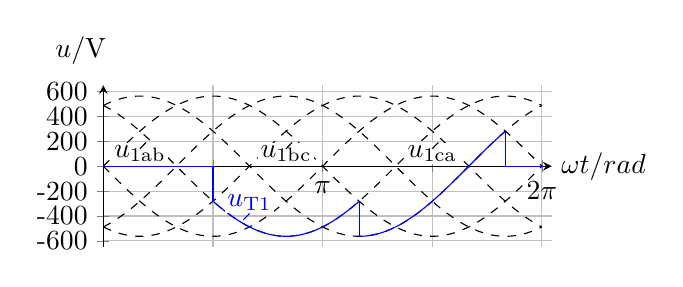
\begin{tikzpicture}
            \begin{axis}[
                % x/y range adjustment
                xmin=0, xmax=368,
                ymin=-650, ymax=650,
                samples=500,
                axis y line=center,
                axis x line=middle,
                extra y ticks=0,
                % Label text
                xlabel={$\omega t / \text{rad}$},,
                ylabel={$u/\mathrm{V}$},
                % Label adjustment
                x label style={at={(axis description cs:1,0.5)},anchor=west},
                y label style={at={(axis description cs:-.05,.97)},anchor=south,yshift=0.2cm},
                width=0.6\textwidth,
                height=0.3\textwidth,
                % x-Ticks
                xtick={0,90,180,270,360},
                xticklabels={,,$\pi$,,$2\pi$},
                xticklabel style = {anchor=north},
                % y-Ticks
                ytick={600,400,200,0,-200,-400,-600},
                yticklabels={600,400,200,0,-200,-400,-600},
                yticklabel style = {anchor=east},
                % Grid layout
                grid,
                %grid style={line width=.1pt, draw=gray!10},
                %major grid style={line width=.2pt,draw=gray!90},
            ]
            % Voltage u1ab(wt), u1bc(wt) u1ca(wt)
            \addplot[black, domain= 0:360,dashed] {563*cos(x-30)};                
            \addplot[black, domain= 0:360,dashed] {563*cos(x+210)}; 
            \addplot[black, domain= 0:360,dashed] {563*cos(x+90)};   
            % Voltage -u1ab(wt), -u1bc(wt) -u1ca(wt)
            \addplot[black, domain= 0:360,dashed] {-563*cos(x-30)};                
            \addplot[black, domain= 0:360,dashed] {-563*cos(x+210)}; 
            \addplot[black, domain= 0:360,dashed] {-563*cos(x+90)};
            % Voltage uT1(wt)
            \addplot[blue, domain= 90:210] {-563*cos(x+210)};                
            \addplot[blue, domain= 210:330] {563*cos(x-30)};                
            \addplot[color=blue,solid] coordinates{
                (0, 0)
                (90, 0)
                (90, -282)
            };     
            \addplot[color=blue,solid] coordinates{
                (210, -563)
                (210, -282)
            };     
            \addplot[color=blue,solid] coordinates{
                (330, 282)
                (330, 0)
            };     
            \addplot[color=blue,solid] coordinates{
                (330, 0)
                (360, 0)
            };     

            % Label of u1ab
            \node[black, fill=white, inner sep = 1pt, anchor = south] at (axis cs:30,10) {$u_{\mathrm{1ab}}$};
            % Line to +u1ab
            \draw[thin, black] (30,140) -- (35,190);            
            % Label of u1bc
            \node[black, fill=white, inner sep = 1pt, anchor = south] at (axis cs:150,10) {$u_{\mathrm{1bc}}$};
            % Line to +u1bc
            \draw[thin, black] (150,140) -- (155,190);            
            % Label of u1ca
            \node[black, fill=white, inner sep = 1pt, anchor = south] at (axis cs:270,10) {$u_{\mathrm{1ca}}$};
            % Line to +u1ca
            \draw[thin, black] (270,140) -- (275,190);            
            % Label of uT1
            \node[blue, fill=white, inner sep = 1pt, anchor = south] at (axis cs:120,-380) {$u_{\mathrm{T1}}$};
            % Line to uT1
            \draw[thin, blue] (120,-380) -- (115,-430);
        \end{axis}     
        \end{tikzpicture}
        \caption{Voltage $u_\mathrm{T1}(\omega t)$ for raising load.}
        \label{sfig:ex06_Voltage_u1T_up}
\end{solutionfigure}

    %%%%%%%%%%%%%%%%%%%%%%%%%%%%%%%%%%%%%%%%%%%%%%%%%%%%%%%%%%%%%%%%%%%%%%%%%%
% Signal of uT1 for lowing load
%%%%%%%%%%%%%%%%%%%%%%%%%%%%%%%%%%%%%%%%%%%%%%%%%%%%%%%%%%%%%%%%%%%%%%%%%%
\begin{solutionfigure}[htb]

 %   \documentclass{standalone}
 %   \usepackage{pgfplots}
 %   \pgfplotsset{compat=1.18} % Kompatibilität für neuere Versionen
        \centering
        \begin{tikzpicture}
            \begin{axis}[
                % x/y range adjustment
                xmin=0, xmax=368,
                ymin=-650, ymax=650,
                samples=500,
                axis y line=center,
                axis x line=middle,
                extra y ticks=0,
                % Label text
                xlabel={$\omega t / \text{rad}$},,
                ylabel={$u/\mathrm{V}$},
                % Label adjustment
                x label style={at={(axis description cs:1,0.5)},anchor=west},
                y label style={at={(axis description cs:-.05,.97)},anchor=south,yshift=0.2cm},
                width=0.6\textwidth,
                height=0.3\textwidth,
                % x-Ticks
                xtick={0,90,180,270,360},
                xticklabels={,,$\pi$,,$2\pi$},
                xticklabel style = {anchor=north},
                % y-Ticks
                ytick={600,400,200,0,-200,-400,-600},
                yticklabels={600,400,200,0,-200,-400,-600},
                yticklabel style = {anchor=east},
                % Grid layout
                grid,
                thick
                %grid style={line width=.1pt, draw=gray!10},
                %major grid style={line width=.2pt,draw=gray!90},
            ]
            % Voltage u1ab(wt), u1bc(wt) u1ca(wt)
            \addplot[black, domain= 0:360,dashed] {563*cos(x-30)};                
            \addplot[black, domain= 0:360,dashed] {563*cos(x+210)}; 
            \addplot[black, domain= 0:360,dashed] {563*cos(x+90)};   
            % Voltage -u1ab(wt), -u1bc(wt) -u1ca(wt)
            \addplot[black, domain= 0:360,dashed] {-563*cos(x-30)};                
            \addplot[black, domain= 0:360,dashed] {-563*cos(x+210)}; 
            \addplot[black, domain= 0:360,dashed] {-563*cos(x+90)};
            % Voltage uT1(wt)
            \addplot[signalalpha, domain= 0:90] {563*cos(x-30)};                
            \addplot[signalalpha, domain= 210:330] {-563*cos(x+210)};             
            \addplot[signalalpha, domain= 330:360] {563*cos(x-30)};             
            \addplot[color=signalalpha,solid] coordinates{
                (90, 282)
                (90, 0)
                (210, 0)
                (210, -282)
            };     
            \addplot[color=signalalpha,solid] coordinates{
                (330, 563)
                (330, 282)
            };     
            % Label of u1ab
            \node[black, fill=white, inner sep = 1pt, anchor = south] at (axis cs:30,10) {$u_{\mathrm{1ab}}$};
            % Line to +u1ab
            \draw[black] (30,140) -- (35,190);            
            % Label of u1bc
            \node[black, fill=white, inner sep = 1pt, anchor = south] at (axis cs:150,10) {$u_{\mathrm{1bc}}$};
            % Line to +u1bc
            \draw[black] (150,140) -- (155,190);            
            % Label of u1ca
            \node[black, fill=white, inner sep = 1pt, anchor = south] at (axis cs:270,10) {$u_{\mathrm{1ca}}$};
            % Line to +u1ca
            \draw[black] (270,140) -- (275,190);            
            % Label of uT1
            \node[signalalpha, fill=white, inner sep = 1pt, anchor = south] at (axis cs:60,200) {$u_{\mathrm{T1}}$};
            % Line to uT1
            \draw[signalalpha] (60,310) -- (70,390);
        \end{axis}     
        \end{tikzpicture}
        \caption{Voltage $u_\mathrm{T1}(\omega t)$ for lowering the load.}
        \label{sfig:ex06_Voltage_u1T_down}
\end{solutionfigure}
    
\end{solutionblock}

% Subtask3
\subtask{Calculate the active power $P$, the fundamental reactive power $Q^\mathrm{(1)}$
and the fundamental apparent power $S^\mathrm{(1)}$ for the two considered operating points. Represent $P$, $Q^\mathrm{(1)}$ and $S^\mathrm{(1)}$ in the complex plane.}
\begin{solutionblock}
    \begin{equation}
        \begin{split}
            P_\mathrm{up}&=U_\mathrm{mot} I_\mathrm{mot}=\SI{466}{\volt} \cdot \SI{20}{\ampere}= \SI{9320}{\watt}. \\
            P_\mathrm{down}&=-U_\mathrm{mot} I_\mathrm{mot}=\SI{-466}{\volt} \cdot \SI{20}{\ampere}= \SI{-9320}{\watt}.
        \end{split}
    \end{equation}
    The input voltage $U_\mathrm{1}^\mathrm{(1)}$ corresponds to $U_\mathrm{1}$, so that the apparent power results to
    \begin{equation}
        \begin{split}
            S_\mathrm{up}^\mathrm{(1)}&=3 U_\mathrm{1} \frac{\hat{i}_\mathrm{1a}^\mathrm{(1)}}{\sqrt{2}}=\SI{230}{\volt} \cdot \frac{\SI{22}{\ampere}}{\sqrt{2}}= \SI{10760}{\volt\ampere}. \\
            S_\mathrm{down}^\mathrm{(1)}&=3 U_\mathrm{1} \frac{\hat{i}_\mathrm{1a}^\mathrm{(1)}}{\sqrt{2}}=\SI{230}{\volt} \cdot \frac{\SI{22}{\ampere}}{\sqrt{2}}= \SI{10760}{\volt\ampere}.
        \end{split}
    \end{equation}
    The reactive power is calculated by
    \begin{equation}
        \begin{split}
            Q_\mathrm{up}^\mathrm{(1)}&=3 U_\mathrm{1} \frac{\hat{i}_\mathrm{1a}^\mathrm{(1)}}{\sqrt{2}} \sin{(\alpha_\mathrm{up})}
            =\SI{230}{\volt} \cdot \frac{\SI{22}{\ampere}}{\sqrt{2}}\sin{(\frac{\pi}{6})}= \SI{5380}{\volt\ampere}. \\
            Q_\mathrm{down}^\mathrm{(1)}&=3 U_\mathrm{1} \frac{\hat{i}_\mathrm{1a}^\mathrm{(1)}}{\sqrt{2}} \sin{(\alpha_\mathrm{down})}
            =\SI{230}{\volt} \cdot \frac{\SI{22}{\ampere}}{\sqrt{2}}\sin{(\frac{5\pi}{6})}= \SI{5380}{\volt\ampere}.
        \end{split}
    \end{equation}
    
    \autoref{sfig:ex06_Complex_Plane_Power} shows the power in the complex plane.

    %%%%%%%%%%%%%%%%%%%%%%%%%%%%%%%%%%%%%%%%%%%%%%%%%%%%%%%%%%%%%%%%%%%%%%%%%%
% Signal of uT1 for raising load
%%%%%%%%%%%%%%%%%%%%%%%%%%%%%%%%%%%%%%%%%%%%%%%%%%%%%%%%%%%%%%%%%%%%%%%%%%
\begin{solutionfigure}[htb]
        \centering
        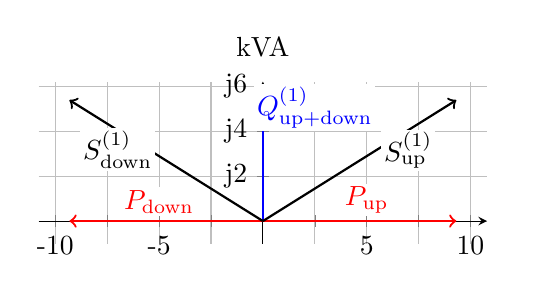
\begin{tikzpicture}
            \begin{axis}[
                % x/y range adjustment
                xmin=-10.8, xmax=10.8,
                ymin=-1000, ymax=6200,
                samples=500,
                axis y line=center,
                axis x line=middle,
                extra y ticks=0,
                % Label text
                xlabel={$\SI{}{\kilo\watt}$},,
                ylabel={$\mathrm{kVA}$},
                % Label adjustment
                x label style={anchor=west},
                y label style={anchor=south,yshift=0.2cm},
                width=0.6\textwidth,
                height=0.3\textwidth,
                % x-Ticks
                xtick={10,7.5,5,2.5,0,-2.5,-5,-7.5,-10},
                xticklabels={10,,5,,,,-5,,-10},
                xticklabel style = {anchor=north},
                % y-Ticks
                ytick={6000,4000,2000,0},
                yticklabels={j6,j4,j2,},
                yticklabel style = {anchor=east},
                extra y ticks = {0},
                extra y tick labels = {},
                % Grid layout
                grid,
                %grid style={line width=.1pt, draw=gray!10},
                %major grid style={line width=.2pt,draw=gray!90},
                ]
                % Q1/2
                \draw[->,blue, solid, thick] (axis cs:0,0) -- (axis cs:0,5380);
                % Label of Qup/down
                \node[blue, fill=white, inner sep = 1pt, anchor = south] at (axis cs:2.5,4000) {$Q_\mathrm{up+down}^\mathrm{(1)}$};
                %Pup
                \draw[->,red, solid, thick] (axis cs:0,0) -- (axis cs:9.320,0);
                % Label of Pup
                \node[red, fill=white, inner sep = 1pt, anchor = south] at (axis cs:5,200) {$P_\mathrm{up}$};
                %Pdown
                \draw[->,red, solid, thick] (axis cs:0,0) -- (axis cs:-9.320,0);
                % Label of Pup
                \node[red, fill=white, inner sep = 1pt, anchor = south] at (axis cs:-5,200) {$P_\mathrm{down}$};
                %Sup
                \draw[->, solid, thick] (axis cs:0,0) -- (axis cs:9.320,5380);
                % Label of Pup
                \node[fill=white, inner sep = 1pt, anchor = south] at (axis cs:7,2200) {$S_\mathrm{up}^\mathrm{(1)}$};
                %Sdown
                \draw[->, solid, thick] (axis cs:0,0) -- (axis cs:-9.320,5380);
                % Label of Pup
                \node[fill=white, inner sep = 1pt, anchor = south] at (axis cs:-7,2200) {$S_\mathrm{down}^\mathrm{(1)}$};
            \end{axis}
        \end{tikzpicture}
        \caption{Power within the complex plane.}
        \label{sfig:ex06_Complex_Plane_Power}
\end{solutionfigure}

\end{solutionblock}

% Subtask4
\subtask{Calculate the fundamental current ratio $g=\frac{I^\mathrm{(1)}}{I}$ and the power factor $\lambda$ for the two considered operating points.}
\begin{solutionblock}
    The fundamental current ratio results to
    \begin{equation}
        g=\frac{\frac{\hat{i}_\mathrm{1a}^\mathrm{(1)}}{\sqrt{2}}}{I_\mathrm{mot}}=\frac{\frac{\SI{22}{\ampere}}{\sqrt{2}}}{\SI{20}{\ampere}}=0.78.
    \end{equation}
    The power factor $\lambda$ is calculated by
    \begin{equation}
        \begin{split}
            \lambda_\mathrm{up}&=g \cdot \cos{(\alpha_\mathrm{up})}=0.78  \cdot \cos(\frac{\pi}{6})= 0.68. \\
            \lambda_\mathrm{down}&=g \cdot \cos{(\alpha_\mathrm{down})}=0.78  \cdot \cos(\frac{5\pi}{6})= -0.68.
        \end{split}
    \end{equation}
\end{solutionblock}
